\chapter{Docker-Anwendungsszenarien für den Softwareentwickler}
\label{cha:szenarien}
Dieses Kapitel zeigt exemplarisch mögliche Anwendungsfälle für die Verwendung von Docker als Werkzeug für Softwareentwickler und wie diese bei ihren alltäglichen Tätigkeiten unterstützen werden können.

Das Entwickeln von Software erfordert die Installation zahlreicher Werkzeuge.
Wenn sich diese auf lediglich ein Projekt beschränkt, stellt dies kein Problem dar, da es zu keinen Versionsinkompatibilitäten kommt und die Werkzeuge nicht laufend gewechselt werden müssen.
Werden allerdings mehrere Projekte parallel entwickelt und zusätzlich noch Beiträge zu Open-Source-Projekten geleistet, wird dieses Unterfangen erheblich komplizierter.
Unterschiedliche Laufzeitumgebungen, Compiler-Versionen, Build-Werkzeuge und Frameworks führen sehr schnell zu einem unüberschaubaren und instabilen System \autocite{smashing-local-devenv-docker:online}.

In \autocite{smashing-local-devenv-docker:online} werden die bestehenden Lösungen für die auftretenden Probleme aufgelistet:
\begin{itemize}
    \item Anstatt Abhängigkeiten auf Systemebene zu installieren werden diese von \emph{Paketmanagern} auf Projektebene verwaltet.
    Vertreter davon sind zum Beispiel npm\footnote{\url{https://www.npmjs.com/}} für JavaScript, Maven\footnote{url{https://maven.apache.org/}} für Java oder NuGet\footnote{\url{https://www.nuget.org/}} für .NET.
    \item Zusätzlich zu Paketen müssen allerdings auch die Laufzeitumgebungen verwaltet werden.
    Bei unterschiedlichen Projekten können unterschiedliche Versionen dieser benötigt werden, wodurch Werkzeuge wie der Node Version Manager (nvm\footnote{\url{https://github.com/creationix/nvm}}) oder der Ruby Version Manager (RVM\footnote{\url{https://rvm.io/}}) entstanden sind.
    Diese müssen allerdings auf dem Entwicklerrechner verwaltet werden und erschweren den schnellen Wechsel zwischen unterschiedlichen Projekten.
    Bei alten Legacy-Systeme ist eine Unterstützung durch diese Werkzeuge außerdem nicht garantiert.
    \item Mit dem Aufschwung der Virtualisierung und Werkzeugen wie Vagrant wurden viele dieser Probleme gelöst.
    Allerdings ist die Notwendigkeit einer virtuellen Maschine pro Projekt sehr ressourcen- und wartungsintensiv.
    Ein weiterer Nachteil ist, dass Vagrant auf Entwicklerrechner ausgelegt ist und dadurch nicht garantiert werden kann, dass die entwickelte Software auch auf dem Produktionssystem läuft \autocite{laradock-docs:online}.
\end{itemize}
Docker bietet eine Abstraktion des Betriebssystems und die Möglichkeit, die benötigten Komponenten einer Anwendung deklarativ zu beschreiben.
Dadurch ist es möglich, die Laufzeitumgebung und die benötigten Komponenten der Anwendung gemeinsam mit dieser im Versionsverwaltungssystem aufzubewahren.
Danach ist lediglich Docker die Voraussetzung dafür, dass mit einem plattformübergreifenden Kommando mit der Entwicklung von Software begonnen werden kann.

Travis Reeder liefert in seinem Blogeintrag über die Entwicklung mit Docker (\autocite{why-docker-for-development:online}) folgende Gründe für die Verwendung von Docker für Softwareentwickler:
\begin{itemize}
    \item Die Entwicklungsumgebung ist nicht vom Betriebssystem oder dessen Version abhängig. Unterschiedliche Personen im Team können problemlos auf Windows, macOS und Linux gemeinsam an einem Produkt arbeiten. Dieser Aspekt ist besonders bei der Entwicklung von Open-Source-Projekten wichtig, da dort unzählige Entwickler ohne zentrale Verwaltung zu einem Produkt beitragen.
    \item Die Entwicklungs- und Produktionsumgebung werden vereinheitlicht. Quelltext, der in der Entwicklungsumgebung getestet ist, funktioniert automatisch auch auf dem Produktivsystem.
    \item Komplizierte Build-Prozesse können abstrahiert werden, sodass die Entwickler diesen nicht verstehen müssen. Außerdem kann dieser Prozess separat entwickelt und getestet oder sogar wiederverwendet werden.
    \item Unterschiedliche Laufzeitumgebungen haben keinen Einfluss auf das Hostsystem des Entwicklers. Besonders die Entwicklung von Java, Ruby, Python und Node wird dadurch stark vereinfacht. Zusätzlich ist es beispielsweise einfach möglich, die Software mit einer anderen Compiler-Version zu übersetzen, um zu überprüfen, ob diese kompatibel ist.
    \item Das Veröffentlichen der Software wird einfacher. Es muss lediglich ein Container der Anwendung erstellt werden, der nun auf jedem Docker-Host lauffähig ist.
    \item Es müssen keine besondere IDE verwendet oder Kommandos über SSH auf einer virtuellen Maschine ausgeführt werden. Der Container wird in das Host-System integriert und ist beinahe nicht sichtbar.
    \item Entwicklern wird ein schnellerer und einfacher Einstieg in ein Projekt ermöglicht, da große Teile des Entwicklungsprozesses abstrahiert werden. Diese muss der Entwickler anfangs nicht verstehen, wodurch die Lernkurve und dadurch auch die Einarbeitungszeit sinken.
\end{itemize}


\section{Softwareevaluierung}
\label{sec:softwareevaluierung}
Die Evaluierung und Auswahl von Werkzeugen, Frameworks und Komponenten eines Softwaresystems ist eine wichtige Aufgabe des Softwareentwicklers.
Ein sehr mühsamer Aspekt dieser Tätigkeit ist das Einarbeiten und Verstehen der Installation und Konfiguration der zu evaluierenden Werkzeuge.
Außerdem werden oftmals unnatürliche Standardpfade (beispielsweise \verb$C:\xampp$ bei der Installation der PHP-Umgebung xampp\footnote{\url{https://www.apachefriends.org/}}) gewählt, oder die Deinstallation von getesteten Werkzeugen hinterlässt Spuren am Host-System des Softwareentwicklers.
Ein weiteres Problem können fehlende Benutzerrechte darstellen, wodurch die Evaluierung bestimmter Werkzeuge gar nicht möglich ist.

\subsubsection{Beispiel: ArangoDB}
Docker ermöglich ein sehr schnelles Testen von Datenbanken, Anwendungsservern und anderen Werkzeugen.
Außerdem wird beim Löschen eines Containers das System automatisch wieder auf einen "`sauberen"' Ausgangszustand zurückgesetzt.
Diese Möglichkeit kann sogar zu Marketingzwecken verwendet werden, wie auf der Homepage von ArangoDB\footnote{\url{https://www.arangodb.com/}} in \cref{fig:arangodb-docker-marketing} dargestellt ist.

Das dort verwendete Kommando ist aus Marketinggründen allerdings etwas zu einfach gehalten.
Würde der Container auf diese Weise gestartet werden, wäre der Netzwerk-Port auf dem Host-System nicht sichtbar und es kann kein Zugriff auf die Datenbank stattfinden.
In \cref{lst:docker-run-arangodb} ist das komplette Startkommando dargestellt.
\cref{fig:arangodb-demo} zeigt die Administrationsoberfläche der gestarteten Datenbank.

Sobald der Container gestoppt wird, wird er durch \texttt{--rm} wieder gelöscht und es verbleiben keine Reste aus der Evaluierungsphase auf dem Host-System.
Ein zusätzlicher Vorteil der Verwendung von Docker ist, dass genau derselbe Container auch im Produktivsystem verwendet werden kann.
Dies ermöglicht beispielsweise die rasche Weiterentwicklung von Prototypen.

\begin{figure}[htbp]
    \centering
    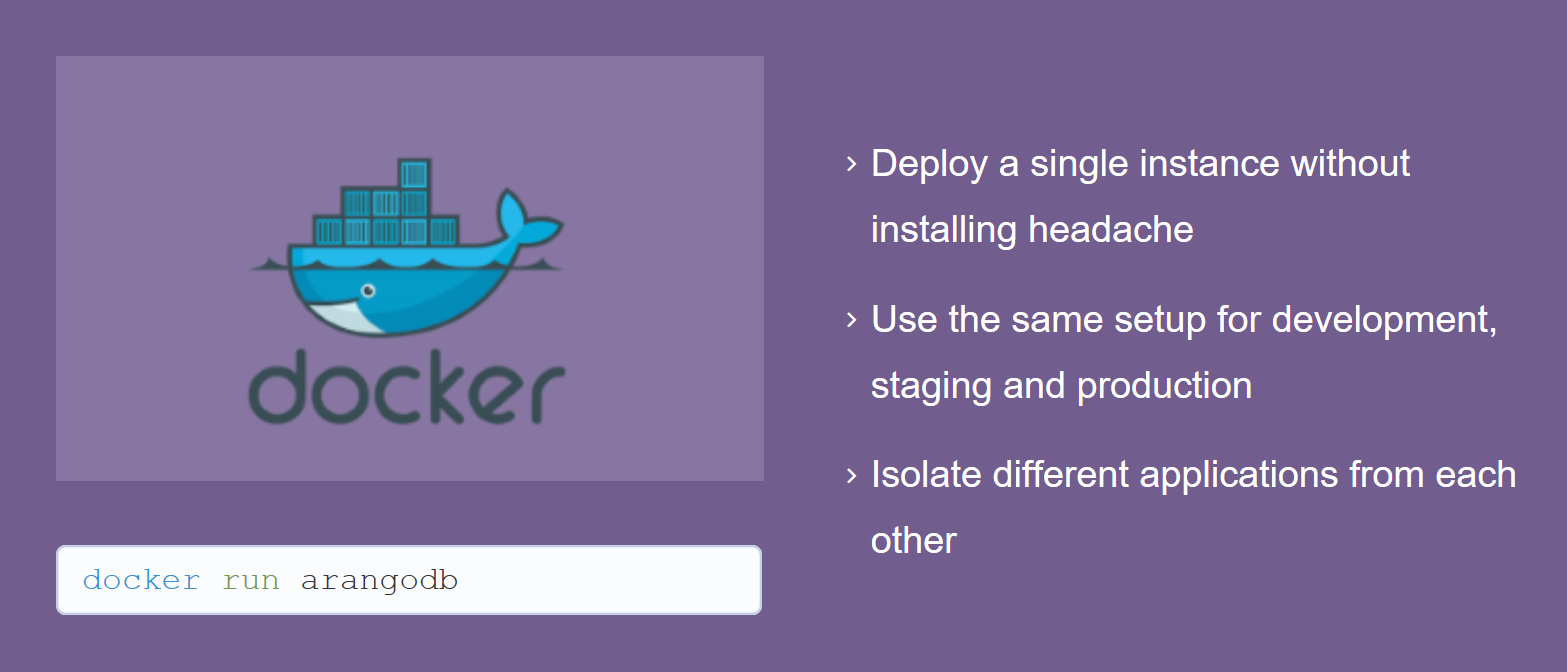
\includegraphics[width=0.7\linewidth,clip]{images/arangodb-docker-marketing}
    \caption{Docker als Marketinginstrument bei ArangoDB}
\label{fig:arangodb-docker-marketing}
\end{figure}

\begin{lstlisting}[caption=Docker-Kommando zum Starten von ArangoDB, language=bash, label=lst:docker-run-arangodb]
docker run --rm -d -e ARANGO_NO_AUTH=1 -p 8529:8529 arangodb
\end{lstlisting}

\begin{figure}[htbp]
    \centering
    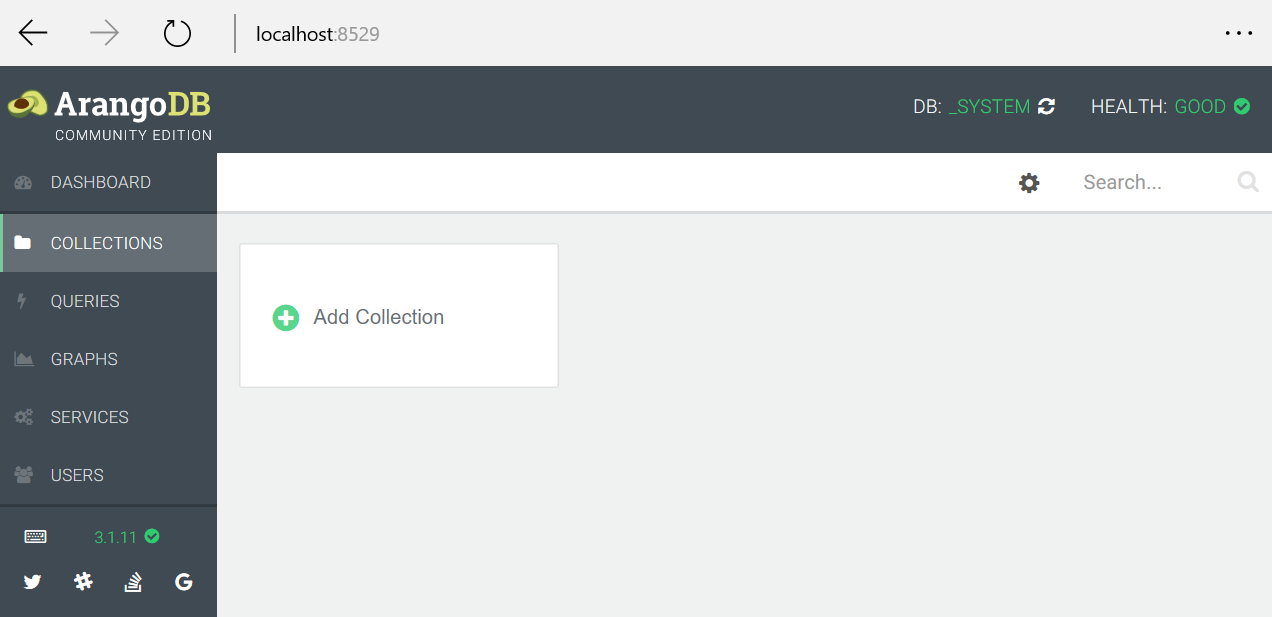
\includegraphics[width=0.9\linewidth,clip]{images/arangodb-demo}
    \caption{ArangoDB als Docker-Container}
\label{fig:arangodb-demo}
\end{figure}

\section{Plattformunabhängige CLI-Anwendungen}
\label{sec:cross-platform-applications}
In \autocite{docker-cli-tools:online} beschreibt Mike English die Möglichkeit, Docker als Laufzeitumgebung für Kommandozeilenwerkzeuge zu verwenden.
Durch die Kombination des Werkzeuges mitsamt seinen Abhängigkeiten werden bei der Verwendung von Docker keine Laufzeitsysteme auf dem Host benötigt.
Dies führt besonders bei Python und Ruby zur Vermeidung von Versionsproblemen und der einfacheren Verwendung auf Windows.
Außerdem bietet Docker mit dem Docker Hub eine sehr angenehme Möglichkeit für die Veröffentlichung und Verbreitung.
Dem gegenüber stehen die Nachteile der Notwendigkeit der Installation von Docker und die damit verbundene Imagegröße aufgrund der Docker-Basisimages.

\subsubsection{Beispiel: Jekyll}
Jekyll\footnote{\url{https://jekyllrb.com/}} ist ein in Ruby geschriebener Generator für statische Webseiten.
In der offiziellen Dokumentation ist beschrieben, dass Windows keine offiziell unterstützte Plattform ist, es aber trotzdem folgende Möglichkeit zur Installation gibt \autocite{jekyll-windows:online}:
\begin{enumerate}
    \item Installieren eines Paketmanagers wie beispielsweise Chocolatey\footnote{\url{https://chocolatey.org/}}.
    \item Installieren von Ruby mit Chocolatey: \texttt{choco install ruby -y}.
    \item Installieren von Jekyll: \texttt{gem install jekyll}.
\end{enumerate}
Für die Installation eines Werkzeuges werden also zwei weitere Werkzeugen benötigt, wobei die Plattform weiterhin als "`nicht offiziell unterstützt"' gilt.

Allerdings bietet Jekyll auch ein vorgefertigtes offizielles Docker-Image\footnote{\url{https://hub.docker.com/r/jekyll/jekyll/}} an, welches mit dem in \cref{lst:docker-run-jekyll} beschriebenen Kommando Jekyll im aktuellen Ordner startet.
Danach ist die Webseite unter \url{http://localhost:4000} erreichbar.

Die Verwendung von Jekyll kann auf diese Weise anstatt der dreistufigen Installation auf das Starten eines Containers reduziert werden.

\begin{lstlisting}[caption=Docker-Kommando zum Starten von Jekyll, language=bash, label=lst:docker-run-jekyll]
docker run -it --rm -v ${pwd}:/srv/jekyll -p 4000:4000 jekyll/jekyll /usr/local/bin/jekyll serve
\end{lstlisting}

\subsubsection{Beispiel: mdp}
Im vorigen Beispiel (Jekyll) diente ein bereits existierendes Docker-Image als Basis für ein plattformunabhängiges Werkzeug.
Da allerdings nicht für jedes Werkzeug ein Docker-Image existiert, ist in \cref{lst:dockerfile-mdp} ein Dockerfile abgebildet, der die Portierung eines existierenden Werkzeuges für Docker zeigt.

\lstinputlisting[caption=Docker-Image für mdp,label={lst:dockerfile-mdp}]{listings/Dockerfile.mdp}
In \cref{lst:dockerfile-mdp} wird ein Docker-Image für mdp\footnote{\url{https://github.com/visit1985/mdp}} erstellt, dieses Verfahren kann aber auf jedes Linux-Kommandozeilenwerkzeug angewendet werden.

mdp ist ein C-Programm, das aus Markdown-Dateien Folien für die Kommandozeile erstellt.
Im Dockerfile werden, wie in der offiziellen Dokumentation beschrieben, die Übersetzung und Installation mit \texttt{make} durchgeführt.
Das Startkommando ist auf eine möglichst intuitive Verwendung ausgelegt (vgl. \cref{sec:container-startup-command}).
Wird keine Präsentationsdatei übergeben, startet der Container mit einer Demo-Präsentation, die die Verwendung von mdp erklärt.


\subsubsection{Aufruf aus der Powershell}
Die Abstraktion von Kommandozeilenanwendungen mit Docker bietet, wie in den beiden Beispielen gesehen, zahlreiche Vorteile.
Doch ein komplettes Docker-Run-Kommando zum Starten einer Anwendung ist nicht nur sehr umständlich und fehleranfällig, sondern verlangt auch bei jedem Start die Konfiguration zahlreicher Parameter.

Dieses Problem lässt sich unter der Verwendung von Shell-Aliasen oder Powershell-Funktionen lösen.
In \cref{lst:powershell-functions} sind die zwei Funktionen zum vereinfachten Starten von Jekyll und mdp aufgelistet.
\texttt{-v \$\{pwd\}:<container-path>} ermöglicht dem Container das Arbeiten mit dem aktuellen Ordner, indem es diesen an den Container bindet.
Mithilfe von \texttt{\$\{args\}} werden die Parameter des Funktionsaufrufes an das Docker-Run-Kommando weitergeleitet.

Der Aufruf der Werkzeuge erfolgt nun wie gewohnt, wobei die Ausführung in einem Docker-Container für den Anwender unsichtbar ist.

\begin{lstlisting}[caption=Powershell-Funktionen für Docker-Kommandos, language=bash, label=lst:powershell-functions]
$ jekyll
function jekyll { docker run -it --rm -v ${pwd}:/srv/jekyll -p 4000:4000 jekyll/jekyll /usr/local/bin/jekyll ${args} }
function mdp { docker run -it --rm -v ${pwd}:/data bemayr/mdp mdp ${args} }
\end{lstlisting}
Ein besonders angenehmer Vorteil bei dieser Shell-Integration ist in \cref{lst:docker-auto-install-cli} dargestellt.
Das Docker-Run-Kommando lädt nicht vorhandene Images vor dem Starten automatisch herunter, wodurch in diesem Fall eine vollautomatische Installation der benötigten Werkzeuge entsteht.
Beim Wechsel oder der Neuinstallation des Host-Systems genügt die Mitnahme der Shell-Konfiguration um das gesamte Werkzeugset auch auf dem neuen System verwenden zu können.
Die Verwaltung der benötigten Werkzeuge erfolgt somit auf einfachste Art und Weise.

\begin{lstlisting}[caption=Automatische Installation der Docker-basierten CLI-Anwendungen, language=bash, label=lst:docker-auto-install-cli]
$ jekyll
Unable to find image 'jekyll/jekyll:latest' locally
latest: Pulling from jekyll/jekyll
baf40e071063: Pull complete
70acac711d95: Downloading [======>          ] 11.33 MB/91.37 MB
...
\end{lstlisting}

\section{Containerbasierte Integrationstests}
\label{sec:containerbasiertes-integrationstests}
Der große Vorteil bei der Verwendung von Containern zum Testen ist ihre Flüchtigkeit.
Durch einen Neustart kann der Ursprungszustand schnell und einfach wiederhergestellt werden.
Unit-Tests profitieren davon nicht, doch die Verwendung von Containern verschafft ihnen eine reproduzierbare und einheitliche Ausführungsumgebung.
Dadurch werden Versionsinkompatibilitäten vermieden und Abhängigkeiten reduziert.

Einen wesentlich größeren Einfluss haben flüchtige Container auf die Ausführung von Integrationstests.
Diese haben aufgrund der zu testenden Komponenten sehr viele Abhängigkeiten wie externe Services, Werkzeuge zum Validieren der Tests (CURL) oder Datenbanken und deren Testdaten.
Um konsistente Testdaten beizubehalten, müssen die Datenbanken vor jedem Testlauf mit diesen neu initialisiert werden.
In containerbasierten Systemen werden die Testdaten automatisch nach jedem Testlauf verworfen, wodurch keine Probleme durch alte Daten auftreten können.
Weiters können externe Services sehr einfach durch zusätzliche Container in das System integriert werden.

Das folgende Beispiel stammt aus \autocite{docker-integration-testing:online}, einem Blogeintrag zum Aufbau eines containerbasierten Integrationstestsystems. Die Architektur dessen ist in \cref{fig:containerbasierte-integrationstests} dargestellt.

\begin{figure}[htbp]
    \centering
    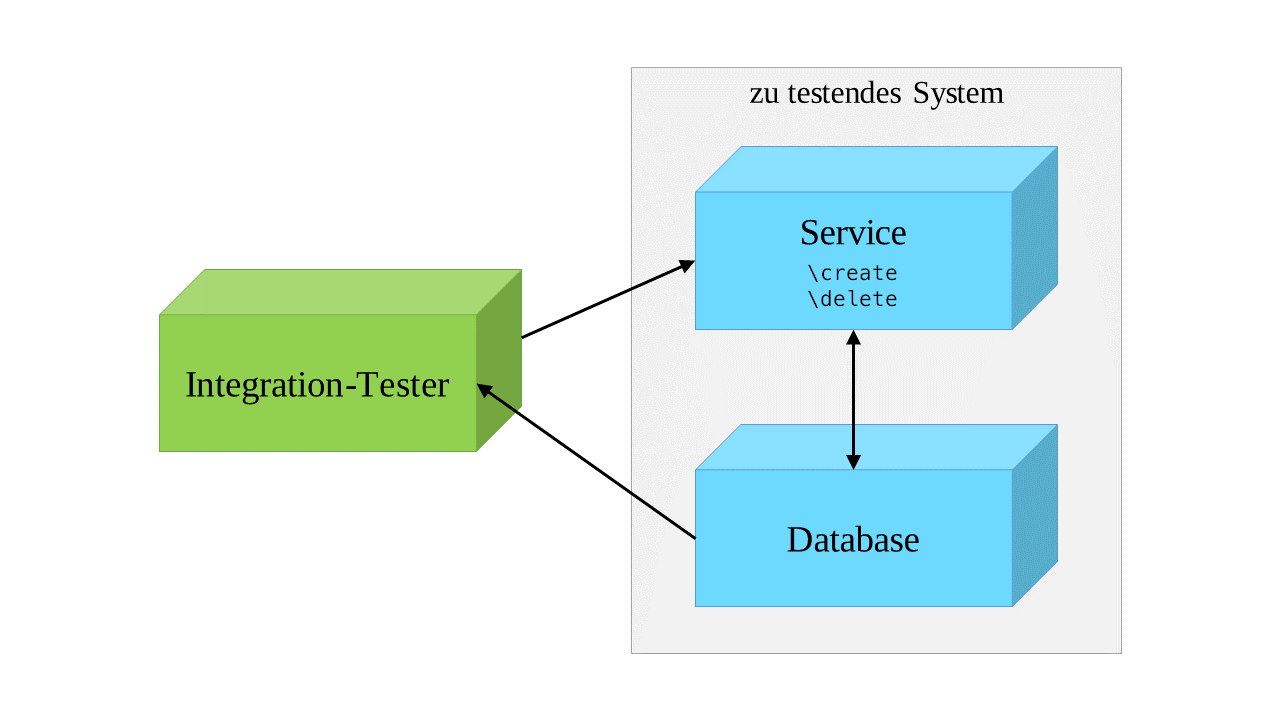
\includegraphics[width=0.7\linewidth,clip,trim=100 30 100 30]{images/containerbasierte-integrationstests}
    \caption{Architektur der containerbasierten Integrationstestsystems \autocite{docker-integration-testing:online}}
\label{fig:containerbasierte-integrationstests}
\end{figure}

\noindent Das zu testende System wird von einem weiteren Container, dem "`Integration-Tester"' gesteuert.
Dieser führt die Testfälle am Service durch und überprüft deren Korrektheit mithilfe von Datenbankabfragen.
Dadurch kann das gesamte System getestet werden, ohne dass Änderungen an diesem oder der dessen Architektur durchgeführt werden müssen.
Dazu muss der Integration-Tester Zugriff auf das Service und die Datenbank haben.
Für den Aufbau dieser Architektur kommt Docker Compose (siehe \cref{sec:docker-compose}) zum Einsatz.
Die Definition der Container ist in \cref{lst:docker-compose-integrationstests} dargestellt.

\begin{lstlisting}[caption=Servicedefinition zum Integrationstesten (docker-compose-yml), label=lst:docker-compose-integrationstests]
version: '2'

services:
  integration-tester:
    build: ./integration-tester
    links:
      - my-service
  my-service:
    build: ./my-service
    command: npm start
    links:
      - rethinkdb
    ports:
      - "8080:8080"
  rethinkdb:
    image: rethinkdb
    expose:
      - "28015"
\end{lstlisting}
Docker-Compose-Dateien definieren im YAML-Format die Parameter, die Docker zum Starten der Container erhält.
In diesem Beispiel werden die in \cref{fig:containerbasierte-integrationstests} definierten Container erstellt und über die Konfigurationsoption \texttt{links} miteinander verbunden.
Der Start der Integrationstests mit \texttt{docker-compose up} führt zu folgendem Ablauf:
\begin{enumerate}
    \item Die Images \emph{my-service} und \emph{integration-tester} werden erstellt.
    \item Die Container \emph{my-service}, \emph{rethinkdb} und \emph{integration-tester} werden gestartet und miteinander verknüpft.
    \item Der Integration-Tester führt die Testfälle aus.
    \item Nach der Fertigstellung der Integrationstests werden die Container gestoppt.
\end{enumerate}

\section{Plattformübergreifende Übersetzung}
\label{sec:plattformuebergreifende-uebersetzung}
Plattformübergreifende Übersetzung ist durch die Idee aus \cref{sec:cross-platform-applications} möglich.
Durch die Möglichkeit, Linux-Anwendungen in Docker-Containern zu starten, können diese nahtlos in Windows eingebunden werden.

\subsubsection{Beispiel: gcc}
In \cref{lst:greet.c} ist ein übliches "`Hello-World"'-Programm in der Programmiersprache C abgebildet.
Um dieses nun auf einem Windows-Host auch unter Linux zu testen, genügt der in \cref{lst:docker-run-gcc} dargestellte Befehl.
Darin wird ein gcc\footnote{\url{https://gcc.gnu.org/}}-Container auf Basis des Alpine-Images zur Übersetzung des C-Programmes verwendet.
In \cref{fig:greet-output} ist das Resultat des Programmes zu sehen, nachdem es in Linux ausgeführt wurde.

Diese Möglichkeit des Cross-Compilings ermöglicht ein schnelles Testen der Plattformunabhängigkeit eines Quelltextes.

\lstinputlisting[caption="`Hello-World"'-C-Programm,label={lst:greet.c}]{listings/greet.c}

\begin{lstlisting}[caption=Docker-Kommando zum Übersetzen eines C-Programmes mit gcc, language=bash, label=lst:docker-run-gcc]
docker run --rm -v ${pwd}:/usr/src -w /usr/src frolvlad/alpine-gcc gcc -o greet greet.c
\end{lstlisting}

\begin{figure}[htbp]
    \centering
    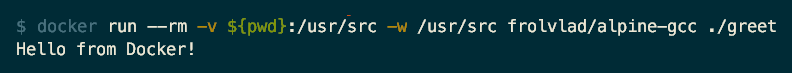
\includegraphics[width=0.8\linewidth,clip]{images/greet-output}
    \caption{Hello-World-Ausgabe unter Linux}
\label{fig:greet-output}
\end{figure}

\subsubsection{Beispiel: dockcross}
Für die plattformübergreifende Übersetzung existieren bereits zahlreiche fertige Docker-Images wie beispielsweise dockcross\footnote{\url{https://github.com/dockcross/dockcross}}.

In \cref{lst:dockercross-arm-greet} sind die notwendigen Kommandos dargestellt, die zum Erstellen des Hello-World-Programms aus \cref{lst:greet.c} für die armv7-Plattform notwendig sind.
In dockcross werden die Container nicht händisch, sondern von einem aus dem Container erzeugbaren Skript ausgeführt.
Dieses Skript wird in Zeile 1 aus dem Container erzeugt, in Zeile 2 werden die notwendigen Berechtigungen gesetzt.

Das Problem dieser Lösung unter Windows ist die fehlende Interpretation der Bash-Kommandos, weshalb die vorgestellten Kommandos unter Docker for Windows in der Powershell nicht ausgeführt werden können.
Für die Ausführung dieses Skriptes unter Windows wird ein Werkzeug wie Cygwin\footnote{\url{https://www.cygwin.com/}}, win-bash\footnote{\url{http://win-bash.sourceforge.net/}} oder Bash on Ubuntu on Windows\footnote{\url{https://msdn.microsoft.com/en-us/commandline/wsl/about}} benötigt.

\begin{lstlisting}[caption=Kommandos zum Übersetzen mit dockcross, language=bash, label=lst:dockercross-arm-greet]
docker run --rm dockcross/linux-armv7 > ./dockcross-linux-armv7
chmod +x ./dockcross-linux-armv7
./dockcross-linux-armv7 bash -c '$CC test/C/greet.c -o greet_arm'
\end{lstlisting}

\section{IDE in a Container}
\label{sec:ideinacontainer}
Der Google-Entwickler Ray Tsang hat die Idee der Entwicklungsumgebung in einem Container\footnote{\url{https://github.com/saturnism/go-ide}} erstmals 2015 vorgestellt \autocite{go-ide-in-a-container:online}.
Der Einsatzzweck seines Containers liegt in der Go-Entwicklung.
Seine Voraussetzungen waren Syntax-Highlighting, Auto-Completion sowie der Zugriff auf die Informationen der Framework-Dokumentation.
Ray Tsang stellt klar, dass seine Idee lediglich ein Experiment ist, definiert jedoch folgende Vorteile einer containerbasierten Entwicklungsumgebung:
\begin{enumerate}
    \item Die Installation der Entwicklungsumgebung dokumentiert sich selbst. Jede Konfiguration wird im Dockerfile festgehalten.
    \item Abhängigkeiten müssen nicht am Host-System, sondern können im Container installiert werden.
    \item Die Entwicklungsumgebung ist portabel. \texttt{docker run ...} genügt zum Starten der IDE auf jedem beliebigen System mit installiertem Docker.
    \item Jeder Entwickler kann seine Anpassungen selbst vornehmen, indem er die deklarative Beschreibung (Dockerfile) des Images ändert.
\end{enumerate}
Ein weiterer Vorteil ist die Möglichkeit der Versionierung der IDE gemeinsam mit dem Projekt.
Dadurch wird Entwicklern ein sehr einfacher Einstieg in ein Projekt ermöglicht.
Außerdem muss für Patches und Fehlerbehebungen in Legacy-Systemen keine eigene alte IDE-Version auf dem Entwicklerrechner behalten werden.

\subsubsection{Beispiel: vim (jare/vim-bundle)}
Eugene Yaremenko\footnote{\url{https://github.com/JAremko}} bietet mit seinen IDE-Containern \emph{jare/vim-bundle}, \emph{jare/drop-in} und \emph{jare/spacemacs} vorkonfigurierte Entwicklungsumgebungen in Docker an.
\cref{fig:vim-demo} zeigt vim\footnote{\url{http://www.vim.org/}} in Docker, das mit dem in \cref{lst:docker-run-vim} dargestellten Kommando gestartet wird.
Für Entwickler, die sich auf der Kommandozeile wohlfühlen, bietet diese Möglichkeit eine sehr portable Entwicklungsumgebung.

\begin{figure}[htbp]
    \centering
    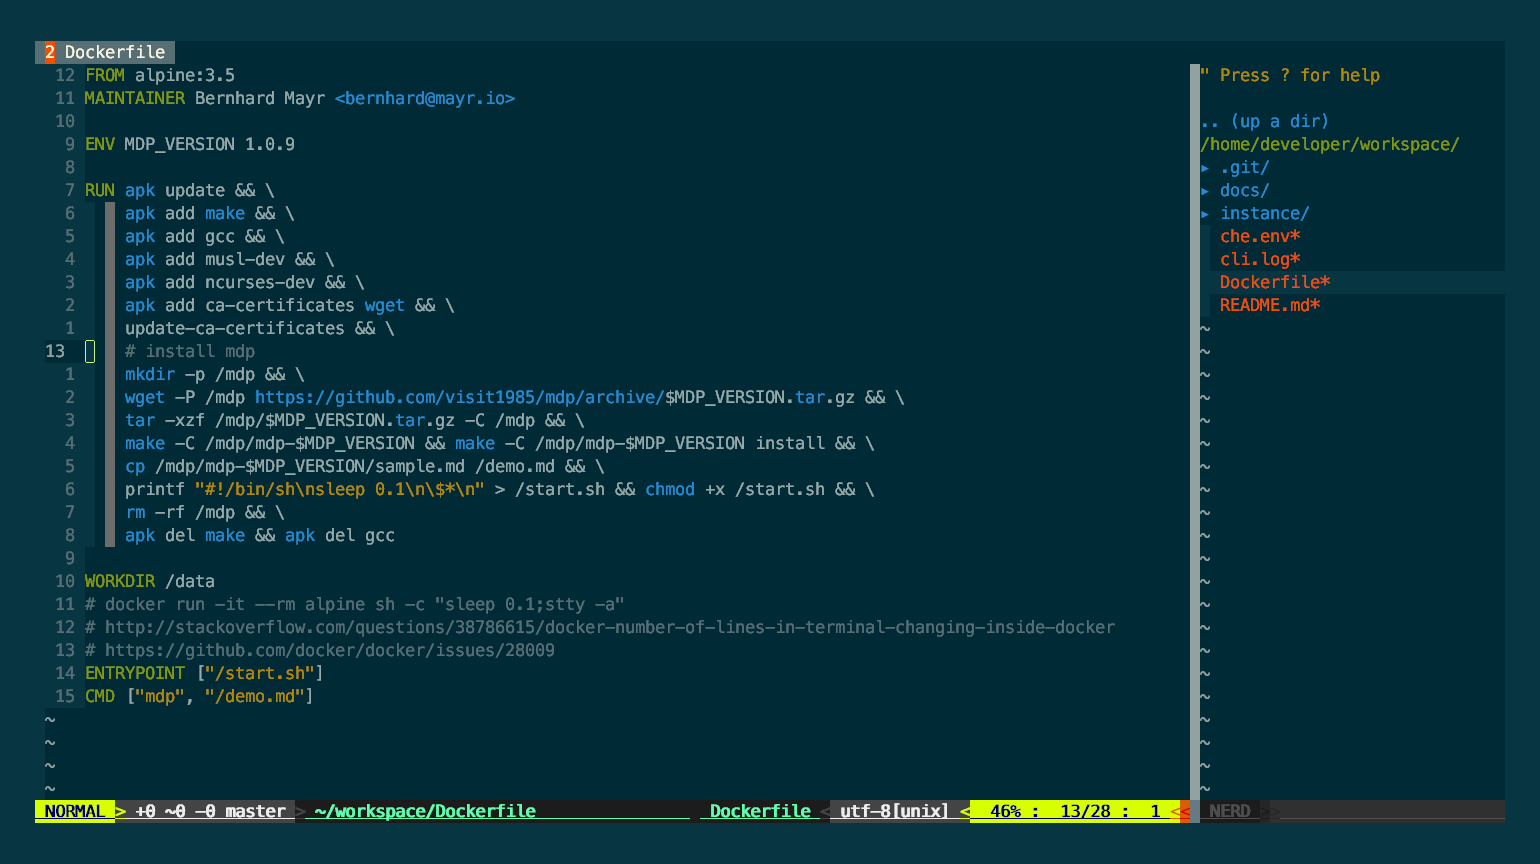
\includegraphics[width=0.9\linewidth,clip]{images/vim-demo}
    \caption{vim als Docker-Container}
\label{fig:vim-demo}
\end{figure}

\begin{lstlisting}[caption=Docker-Kommando zum Starten von vim, language=bash, label=lst:docker-run-vim]
$ docker run -it --rm -v ${pwd}:/home/developer/workspace jare/vim-bundle
\end{lstlisting}

\subsubsection{Beispiel: Eclipse Che}
Einen fundamental anderen Ansatz verfolgt die neue Cloud-IDE Eclipse Che\footnote{\url{http://www.eclipse.org/che/}}.
Deren Grundidee ist die Entwicklung von Software ohne der Installation von Werkzeugen.
Die IDE selbst läuft als Webanwendung und wird über den Browser bedient.
Das gesamte Plug-in-System baut auf Docker-Containern auf, die lediglich kleine Teilaufgaben der Entwicklungsumgebung übernehmen.

In \cref{lst:docker-run-eclipse-che} ist der Startvorgang von Eclipse Che zu sehen.
Dem Container wird der Docker-Socket des Host-Systems übergeben, sodass dieser selbst Container starten und verwalten kann.
Die gestartete IDE ist in \cref{fig:eclipse-che-demo} zu sehen.

\begin{lstlisting}[caption=Docker-Kommando zum Starten von Eclipse Che, language=bash, label=lst:docker-run-eclipse-che]
$ docker run --rm -v /var/run/docker.sock\\:/var/run/docker.sock -v ${pwd}:/data eclipse/che start
WARN: Bound 'eclipse/che' to 'eclipse/che:5.3.1'
INFO: (che cli): 5.3.1 - using docker 1.13.1 / docker4windows
INFO: (che start): Booted and reachable
INFO: (che start): Ver: 5.3.1
INFO: (che start): Use: http://10.0.75.2:8080
INFO: (che start): API: http://10.0.75.2:8080/swagger
\end{lstlisting}

\begin{figure}[htbp]
    \centering
    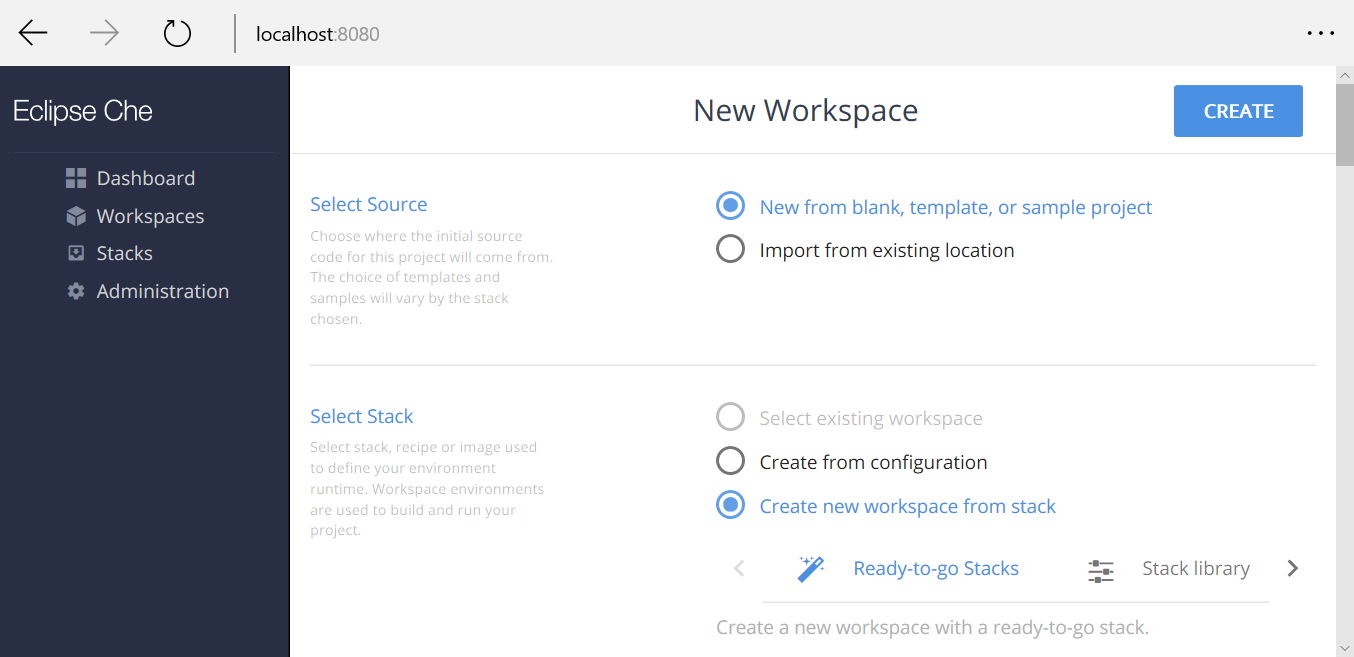
\includegraphics[width=0.9\linewidth,clip]{images/eclipse-che-demo}
    \caption{Eclipse Che als Docker-Container}
\label{fig:eclipse-che-demo}
\end{figure}

% (- https://medium.com/@andyccs/webpack-and-docker-for-development-and-deployment-ae0e73243db4#.dh1mcvvqx)


% ===== EVENTUELL =====
% \section{Docker als Unterstützung zur Entwicklungsumgebung}
% \label{sec:docker-assistance}
%   evtl. SWK6-Umgebung in Docker nachbauen
%   Java, Gradle: http://endoflineblog.com/optimizing-development-with-docker
%   https://blog.nimbleci.com/2016/11/17/whats-coming-in-docker-1-13/
%   http://vuetips.com/use-docker-containers
